\documentclass[dvipdfmx]{standalone}
\usepackage{tikz}
\usepackage{tecfig}
\usepackage{ifthen}
\usetikzlibrary{calc}
\usetikzlibrary{positioning}
\begin{document}
	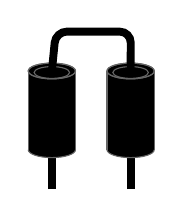
\begin{tikzpicture}
		\newcommand\atama[5]{
			% (x, y, h, a, b)
			\coordinate (a) at (#1, #2);
			\coordinate (a1) at ($(a) + (-#4, 0)$);
			\coordinate (a2) at ($(a) + (+#4, 0)$);
			\coordinate (b1) at ($(a) + (-#4, #3)$);
			\coordinate (b2) at ($(a) + (+#4, #3)$);
			\path[fill=black] (a2) arc (0:-180:#4 and #5) -- ++(0, #3) arc (180:0:#4 and #5) -- cycle;
			\draw[black!60] (a1) -- (b1);
			\draw[black!60] (a2) -- (b2);
			\draw[black!60] (a2) arc (0:-180:#4 and #5);
			\draw[black!60, scale=1] ($(a) + (0, #3)$) ellipse (#4 and #5);
			\draw[black!60] ($(a) + (0, #3)$) ellipse (#4 and #5);
			\draw[black!60, scale=0.75] ($(a) + (0, #3) + (0, #3/3.25)$) ellipse (#4 and #5);
		}
		
		\draw[line width=1mm] (0, -0.5) -- ++(0, 0.5);
		\draw[line width=1mm] (1, -0.5) -- ++(0, 0.5);
		\atama{0}{0}{1.0}{3.0mm}{1.0mm}
		\atama{1}{0}{1.0}{3.0mm}{1.0mm}
		\draw[rounded corners, line width=1mm]
			(0, 1.0) -- (0+0.05, 1.5) -- (1+0.0025, 1.5) -- (1, 1.0);
		
	\end{tikzpicture}
\end{document}
